\documentclass[tikz,border=8pt]{standalone}
% Shared look for every TikZ diagram. Load with \input{../../tools/tikz-style.tex}
\usepackage[T1]{fontenc}
\usepackage{lmodern}
\renewcommand{\sfdefault}{lmr}  % diagrams use the same serif as the text
\usetikzlibrary{arrows.meta, positioning, shapes.geometric, calc, fit, backgrounds}
\definecolor{cblue}{HTML}{4C78A8}
\definecolor{corange}{HTML}{F58518}
\definecolor{cgreen}{HTML}{54A24B}
\definecolor{cred}{HTML}{E45756}
\definecolor{cpurple}{HTML}{B279A2}
\definecolor{cgrey}{HTML}{6B6B6B}
\tikzset{
  every picture/.style={font=\sffamily, line width=1.2pt},
  box/.style={draw=#1, fill=#1!12, rounded corners=4pt, align=center, inner sep=7pt, minimum height=1.1cm},
  box/.default=cgrey,
  arrow/.style={-{Stealth[length=3mm]}, draw=cgrey, line width=1.4pt},
  title/.style={font=\sffamily\bfseries\Large},
  note/.style={font=\sffamily\small, text=cgrey, align=center},
}
\AtBeginDocument{\hyphenpenalty=10000 \exhyphenpenalty=10000}

% Room 5 m x 4 m, robot at A = (2, 2, 0). Landmarks: pink pole (4.4, 3.8), green pole (0.4, 3.2), blue pole (3.2, 0.4).
% Readings (range m, bearing deg): pink (3.10, 40), green (1.95, 141), blue (2.05, -55).
\begin{document}
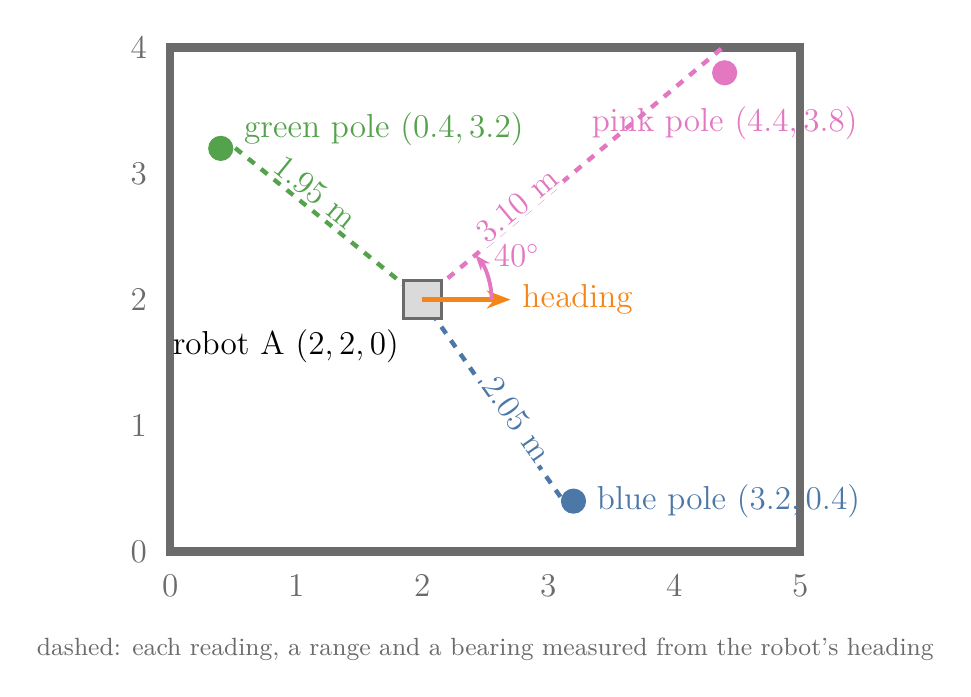
\begin{tikzpicture}[scale=1.6, every node/.append style={font=\large}]
  \draw[cgrey, line width=3pt] (0,0) rectangle (5,4);
  \foreach \x in {0,1,...,5} \node[below, cgrey] at (\x,-0.1) {\x};
  \foreach \y in {0,1,...,4} \node[left, cgrey] at (-0.1,\y) {\y};
  \definecolor{cpink}{HTML}{E377C2}
  % readings as dashed lines from the robot
  \draw[cpink, dashed, line width=1.6pt] (2,2) -- ++(40:3.10);
  \draw[cgreen, dashed, line width=1.6pt] (2,2) -- ++(141:1.95);
  \draw[cblue, dashed, line width=1.6pt] (2,2) -- ++(-55:2.05);
  \fill[cpink] (4.4,3.8) circle (0.1);  \node[cpink, below] at (4.4,3.62) {pink pole $(4.4, 3.8)$};
  \fill[cgreen] (0.4,3.2) circle (0.1); \node[cgreen, right] at (0.5,3.35) {green pole $(0.4, 3.2)$};
  \fill[cblue] (3.2,0.4) circle (0.1);  \node[cblue, right] at (3.3,0.4) {blue pole $(3.2, 0.4)$};
  % robot and heading
  \draw[cgrey, fill=cgrey!25] (1.85,1.85) rectangle (2.15,2.15);
  \draw[-{Stealth[length=3mm]}, corange, line width=2pt] (2,2) -- (2.7,2) node[right] {heading};
  \draw[cpink, line width=1.4pt, -{Stealth[length=2mm]}] (2.55,2) arc (0:40:0.55);
  \node[cpink] at (2.75,2.35) {$40^\circ$};
  \node[cpink, rotate=40, fill=white, inner sep=1pt] at (2.75,2.75) {$3.10$ m};
  \node[cgreen, rotate=-39, fill=white, inner sep=1pt] at (1.15,2.85) {$1.95$ m};
  \node[cblue, rotate=-55, fill=white, inner sep=1pt] at (2.75,1.05) {$2.05$ m};
  \node[below left] at (1.9,1.85) {robot A $(2, 2, 0)$};
  \node[note, anchor=north] at (2.5,-0.6) {dashed: each reading, a range and a bearing measured from the robot's heading};
\end{tikzpicture}
\end{document}
